\chapter{The Hybrid: Cheureg/Tsoureki}
\label{ch:cheureg}
\index{dessert}
\index{bread}
\index{mahleb}
\index{Easter}

\marginnote{
    \textbf{Makes 6 medium braids} \\
    Prep time: 5-6 hours \\
    Cook time: 30-45 minutes \\
    \vspace*{\baselineskip}

    \textbf{Dry ingredients} \\
    2 ¼ tsp instant yeast \\
    2 tsp mahleb \\
    2.5g mastiha, freshly ground \\
    830g AP flour, Robin Hood \\
    267g sugar \\
    1/2 tsp salt \\
    \vspace*{\baselineskip}

    \textbf{Wet ingredients} \\
    84g water, room T \\
    334g whole milk, room T \\
    4 eggs, room T \\

    227g unsalted butter, room T, very soft and cut into cubes \\
    \vspace*{\baselineskip}
        
    \textbf{Before baking} \\
    2 egg yolks and 1 egg white, for egg wash \\
    Slivered almonds 
}

\textit{Easter bread}

Family member: Elsa \& Vaski

\newthought{Our recipe} is based on Vaski's Family Choreg recipe with a few modifications! It contains both mahleb and \textgreek{μαστίχα}. Make sure to use All purpose flour not bread flour, yields a more fluffy \mbox{Cheureg/Tsoureki}.

\begin{enumerate}
    \item In a mixing bowl, whisk the dry ingredients. In another bowl, whisk wet ingredients together. Gradually add wet ingredients to dry ingredients while mixing. Mix for 5 minutes with the paddle. Let rest for a few minutes.
    \item Mix for 5-7 minutes while adding about 90g additional flour until dough comes together and sides start to unstick. Switch to hook attachment. (If dough already has come together don't add any additional flour).
    \item Add 1/3 of the butter and mix until fully incorporated before adding another third. Do the same for the last third of the butter.
    \item Mix on medium until dough is smooth, has unstuck from the sides of the bowl and passes the windowpane test. Approximately 20 minutes of mixing total. Place dough in a bowl, cover with plastic wrap and let rise for 90 minutes in a warm place - in the oven with lights on/oven off works well!
    \item Divide dough into 80g and shape into balls. Shape into small logs and into 6 braids. If you have extra strands you can make individual kaiser buns. Let rise 1 hour to 1 hour and a half. 
    \item Meanwhile, preheat the oven to 350\degree F.
    \item Brush with egg wash and add slivered almonds on top of each braid. Bake for 20 minutes, rotate pans and place another plan under pans (double) and bake for another 7 to 10+ minutes or until brown. Larger braids can be baked for 35 minutes.
    \item Cool, share with family/friends and enjoy with coffee!
\end{enumerate}

\twosidecaptionfigure{velsa/images/PXL_20240331_211621965.PORTRAIT.ORIGINAL.jpg}{velsa/images/PXL_20240331_230346663.PORTRAIT.ORIGINAL.jpg}{Tsoureki/Cheureg hybrid pre and post baking}{fig:cheureg}

\captionfigure{velsa/images/Tsoureki braid_Aki.PNG}{Four-braid braiding instructions}{fig:cheureg_braid}

% \begin{figure}
%   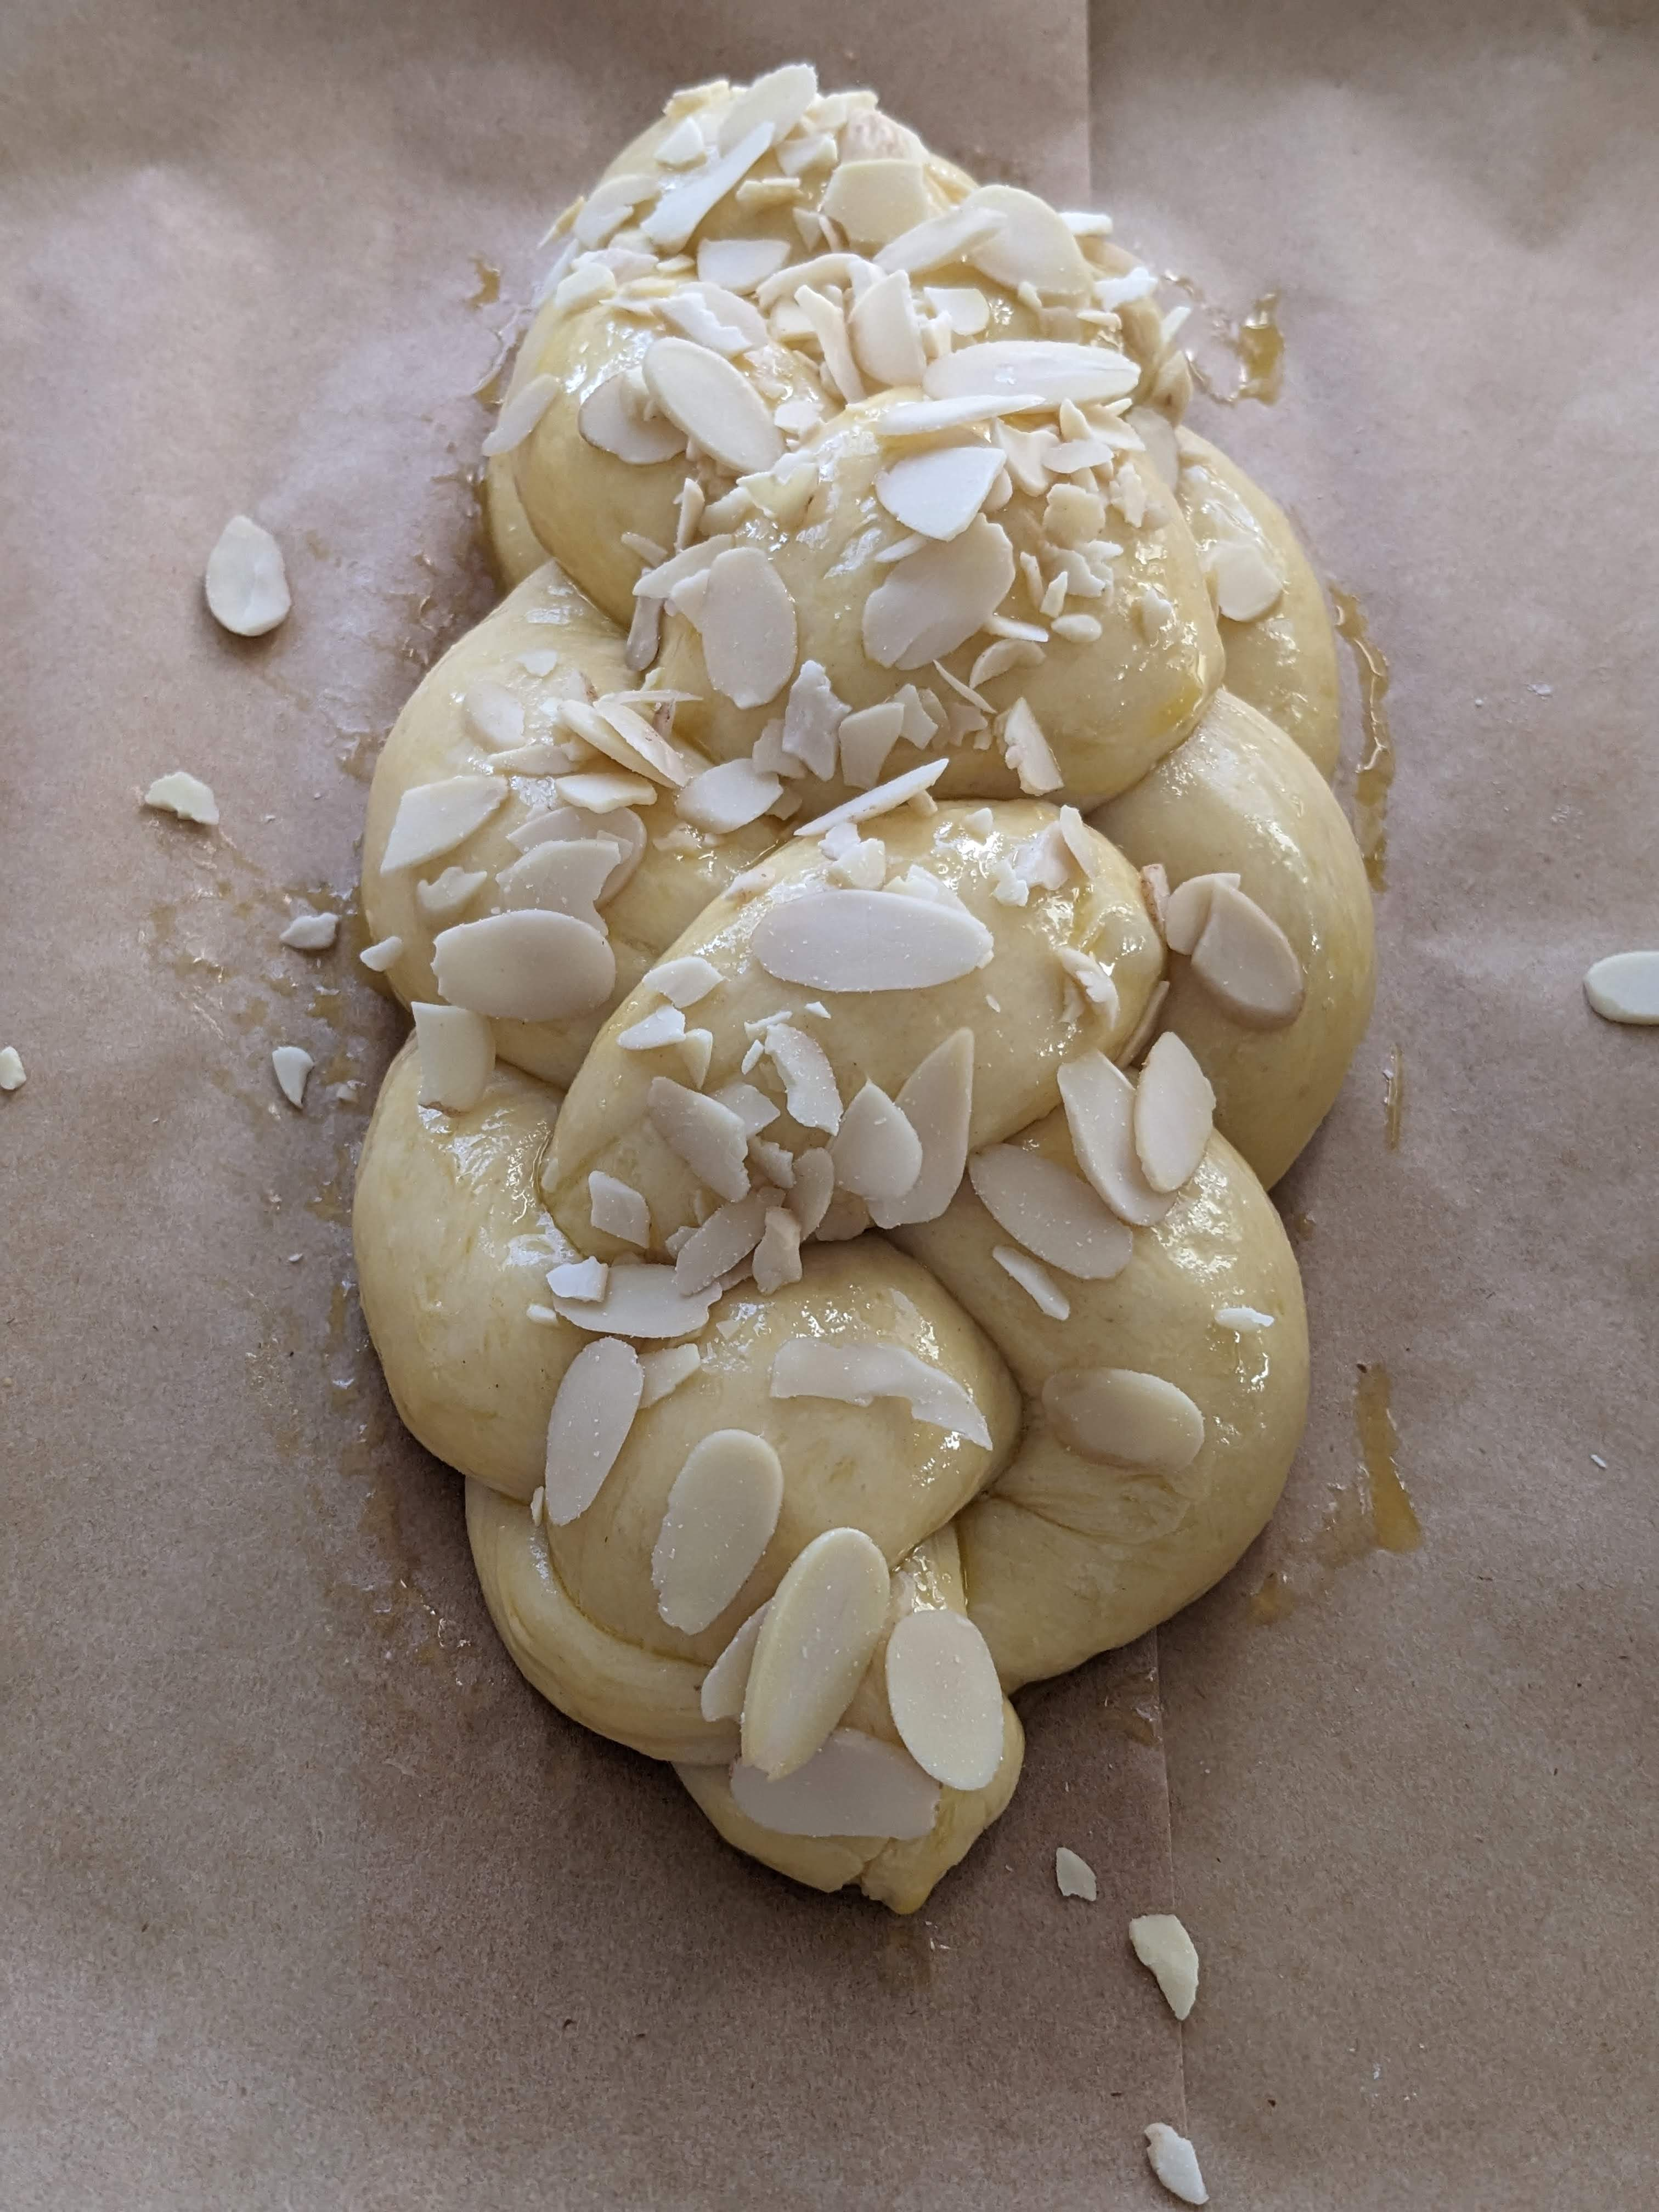
\includegraphics[width=70mm]{velsa/images/PXL_20240331_211621965.PORTRAIT.ORIGINAL.jpg}
% \end{figure}
% \begin{figure}
%   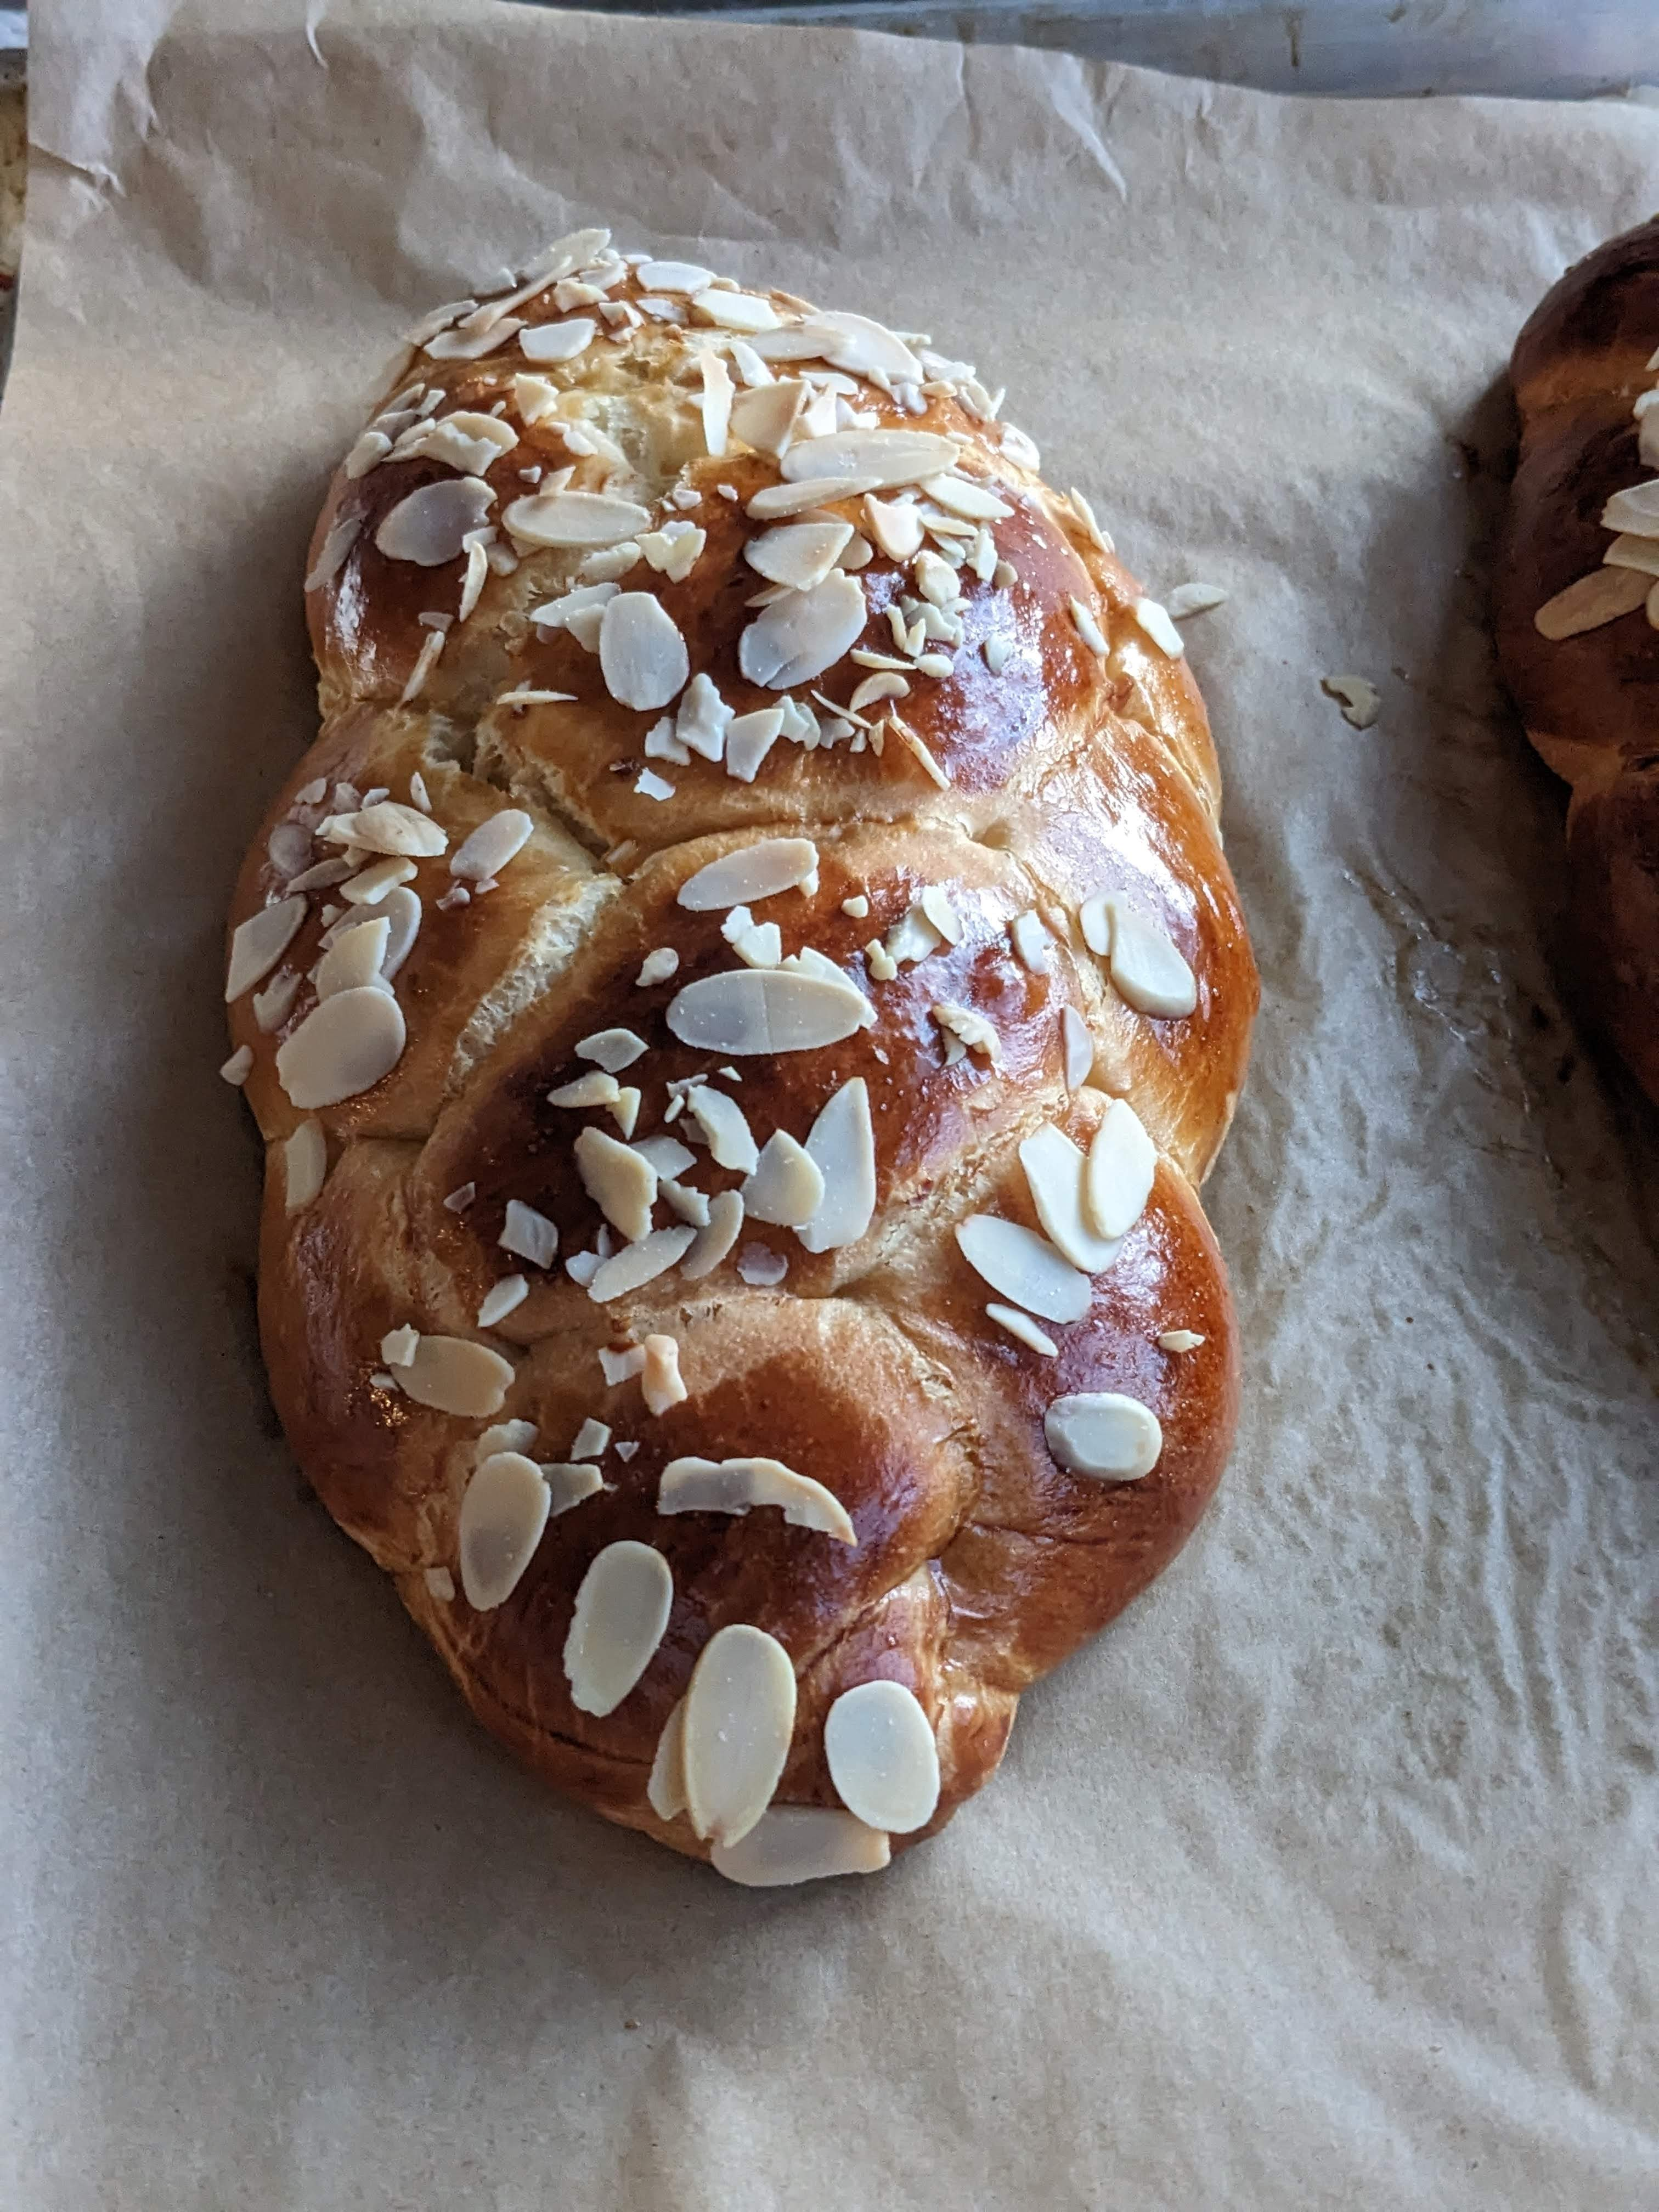
\includegraphics[width=70mm]{velsa/images/PXL_20240331_230346663.PORTRAIT.ORIGINAL.jpg}
% \end{figure}
% \begin{figure}
%   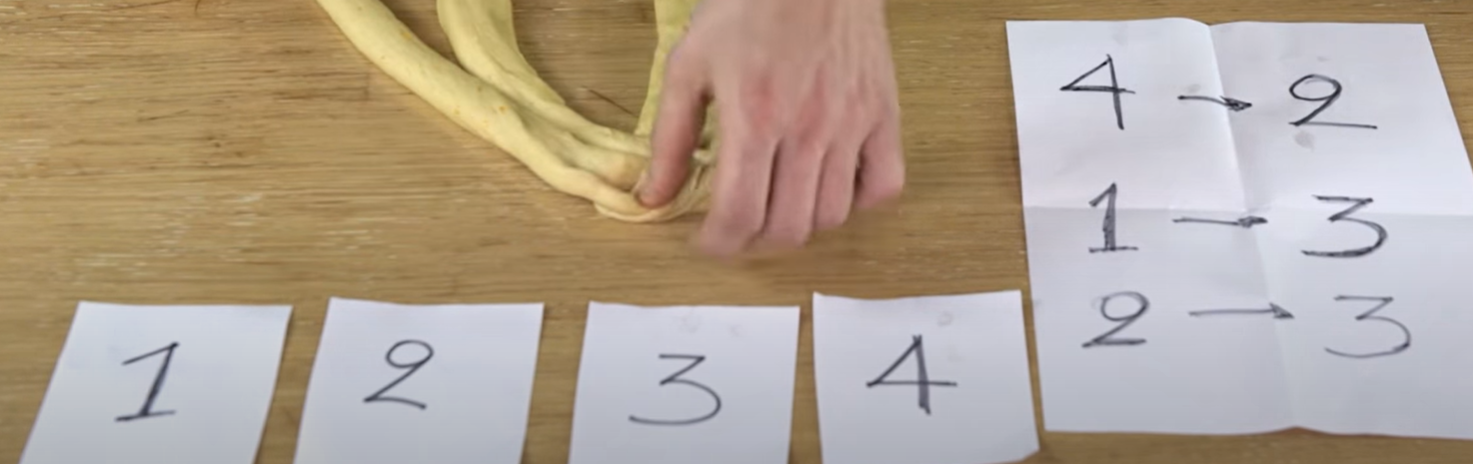
\includegraphics[width=100mm]{velsa/images/Tsoureki braid_Aki.PNG}
% \end{figure}
